\documentclass[10pt,twocolumn]{article}
\usepackage[letterpaper,height=9.0in,width=6.5in,columnsep=0.25in]{geometry}

\usepackage{verbatim}
\usepackage{times}
\usepackage{setspace}
\usepackage{epsfig}
%\usepackage{amssymb}
%\usepackage{amsmath}
%\usepackage{amsfonts}
%\usepackage{amsthm}
\usepackage{xspace}
\usepackage{subfigure}
\usepackage{bibspacing}
\usepackage{color}
\usepackage{url}
\usepackage{hyperref}
\usepackage[small,compact]{titlesec}
\usepackage[footnotesize,bf]{caption}
\usepackage{threeparttable}
\usepackage{tabularx}
\usepackage{booktabs}

\singlespacing

\newcommand{\ie}{i.e.}
\newcommand{\eg}{e.g.}
\newcommand{\PhoneLab}{\textsc{PhoneLab}}

%
%
% Give latex lots of freedom to cram figures onto pages that
% already have figures or text (and not much freedom to create partially
% full pages of only figures)
%
\renewcommand{\textfraction}{0.01}
\setcounter{topnumber}{100}
\setcounter{dbltopnumber}{100}
\setcounter{totalnumber}{100}
\renewcommand{\topfraction}{.9}
\renewcommand{\floatpagefraction}{.9}
\renewcommand{\dbltopfraction}{.9}
\renewcommand{\dblfloatpagefraction}{.9}

%
% Figure stuff
%
\renewcommand{\figurename}{Fig.}

\newcommand{\captionfonts}{\footnotesize}
\setlength{\abovecaptionskip}{0in}
\setlength{\belowcaptionskip}{-.0in}

\hyphenation{Phone-Lab}

\begin{document}
\date{}

\title{Participant Behavior in \textsc{PhoneLab}}

\author{
Anandatirtha Nandugudi, Anudipa Maiti, Fatih Bulut, Sonali Batra, Taeyeon Ki\\
Geoffrey Challen, Murat Demirbas, Steven Y. Ko, Tevfik Kosar, and Chunming
Qiao\\
\\
Department of Computer Science and Engineering\\
University at Buffalo, The State University of New York\\
\href{mailto:team@phone-lab.org}{\nolinkurl{team@phone-lab.org}}
}

\maketitle

\pagestyle{empty}

\section{Introduction}
\label{sec-introduction}

This abstract examines the behavior of the participants in \PhoneLab{}, a public
smartphone testbed being developed at SUNY Buffalo. Currently consisting of 191
participants using Nexus S 4G smartphones, \PhoneLab{} aims to provide a
combination of unique features desirable for smartphone experimentation. This
abstract briefly introduces \PhoneLab{} and presents some of the early results
of a usage measurement study conducted with 115 participants. 

\subsection{\PhoneLab{} Overview}

\PhoneLab{} is designed to provide the following features necessary for
smartphone research---open access, scale, power, realism, locality, and
relevance:

\begin{itemize}
\itemsep -2pt
\item {\bf Open Access:} After the initial approval process, \PhoneLab{} allows
any researcher to deploy their research prototype on the participants'
smartphones.
\item {\bf Scale:} By 2014, \PhoneLab{} will grow to 700 participants already
incentivized and recruited to participate in experiments; participants of
\PhoneLab{} receive discounted voice, data, and messaging.
\item {\bf Power:} By utilizing the Android open-source smartphone platform,
\PhoneLab{} allows application-level experiments as well as platform-level,
i.e., the OS kernel, middleware, and libraries.
\item {\bf Realism:} Participants use the phones as their primary device.
\item {\bf Locality:} Most participants live in Buffalo near SUNY campuses,
enabling research requiring device-to-device interaction.
\item {\bf Relevance:} \PhoneLab{} allows researchers to stop relying on
out-of-date datasets. Instead, new data can be collected in the most
appropriate way for the experiment.
\end{itemize}

\PhoneLab{} application-level experiments are distributed through the Play
Store; participants are notified of new experiments and install the experimental
applications directly from the Play Store. On the other hand, \PhoneLab{}
platform-level experiments are distributed through the \PhoneLab{} control
software that runs on each participant's phone; this control software is capable
of updating platform components, e.g., libraries and kernel modules. To the best
of our knowledge, \PhoneLab{} is the only testbed that provides all the above
features together.

\subsection{\PhoneLab{} Demographics}

Currently, \PhoneLab{} consists of 191 participants. Roughly half of our
participants are first- and second-year undergraduates, a quarter PhD students,
and a fifth faculty, staff and other professionals. However, males greatly
outnumber females, and the young outnumber the middle-aged and older, both
unrepresentative features we will try and rectify in the future years. For
management reasons we limited participation to people with a SUNY Buffalo
affiliation except for several exceptions: a local reporter, a technology
writer, and an international rock star. Table~\ref{tab:demographics} summarizes
our demographics.

\begin{table}[t]
\begin{threeparttable}
\begin{tabularx}{\columnwidth}{Xr@{\hspace{0.5in}}Xr}
\multicolumn{4}{c}{\textbf{Affiliation}} \\
\midrule
Freshman & 64 & Masters & 5 \\
Sophomore & 33 & PhD & 53 \\
Junior & 1 & Faculty/Staff & 29 \\
Senior & 1 & None & 5 \\[0.1in]
\multicolumn{4}{c}{\textbf{Gender}} \\
\midrule
Female & 51 & Male & 140 \\[0.1in]
\multicolumn{4}{c}{\textbf{Age}} \\
\midrule
Under 18 & 12 & 30--34 & 15 \\
18--19 & 74 & 35--39 & 6 \\
20--21 & 12 & 40--49 & 13 \\
22--24 & 22 & 50--59 & 7 \\
25--29 & 29 & 60+ & 1\\
\end{tabularx}
\end{threeparttable}
\caption{Demographic breakdown of 191 \PhoneLab{} participants. Date
ranges are inclusive.}
\vspace{-.2in}
\label{tab:demographics}
\end{table}

\begin{figure*}[t]
\centering
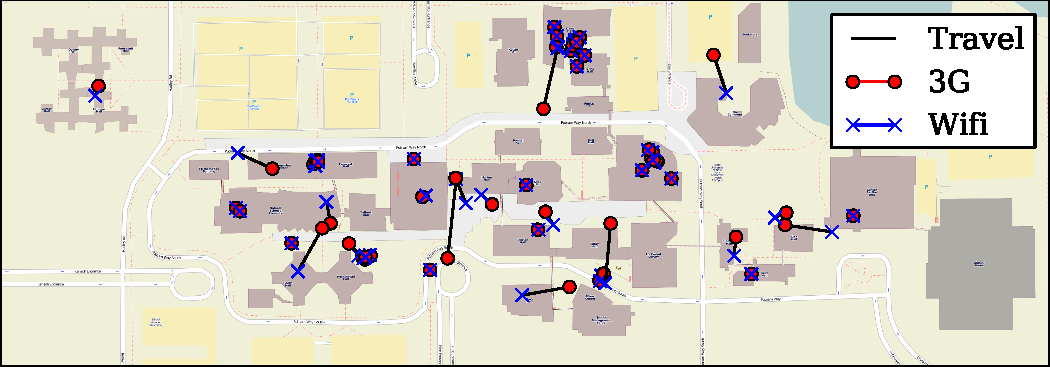
\includegraphics[width=0.8\textwidth]{./figs/network-transitions.pdf}
\caption{\textbf{3G to Wifi transition locations.} The map indicates that
there are several common areas where network hand-offs occur.}
\label{figure-networktransitions}
\end{figure*}

\begin{figure*}[t]
\centering
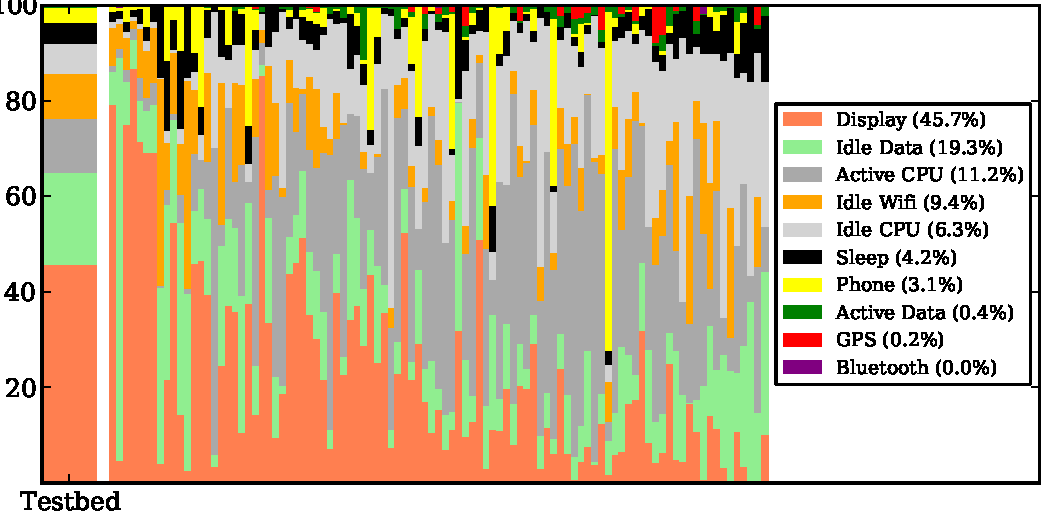
\includegraphics[width=0.7\textwidth]{./figs/battery-breakdown.pdf}
\caption{\textbf{Power usage by component.} The large bar at left shows an
aggregated breakdown for all participants. The participant bars are scaled
against the participant with the most energy usage.}
\label{figure-batteryoverview}
\end{figure*}

\section{Participant Behavior}
\label{sec-usage}

We have conducted a usage measurement study with 115 participants over 21 days.
For this purpose, we have developed a measurement application that collects all
salient features of smartphone usage: networking, mobility, power consumption,
and application usage.

This section presents some of the early results of this study. We show the
network transition behavior between 3G and WiFi first and the battery and
charging behavior next.

\subsection{Mobile Network Transitions}
\label{subsec-networktransitions}

Mobile devices like smartphones move through a complex network environment.
Providing the illusion of seamless connectivity requires negotiating hand-offs
both between Wifi access points and between Wifi and 3G radios. We were
interested in observing hand-offs between 3G (provided by Sprint, \PhoneLab{}'s
operational partner) and Wifi and found many in the dataset collected by our
usage experiment. Since the Android \texttt{ConnectivityService} frequently
switches network interfaces for exploration purposes, we have defined a
transition as two one-minute or longer sessions on different interfaces
separated by less than one minute. We further limit ourselves to cases where we
received a location update during the transition.

Figure~\ref{figure-networktransitions} plots the location of transitions that
occurred on or near SUNY North Campus. We notice that many cluster in
expected locations: near the entrance and exits of buildings where
participants are likely to be moving from campus Wifi to 3G.

\subsection{Energy Breakdown}

A single-day component-by-component breakdown is shown in
Figure~\ref{figure-batteryoverview}. Our results are similar to those reported
by a previous smaller-scale study~\cite{shye:micro:2009}, and indicate that
mobile data (labeled as ``Idle data'' and ``Active data'' depending on the
state), the screen, and CPU usage are the main sources of smartphone power
consumption. The per-participant bars also show a great deal of variation, with
differences in both the amount and the breakdown of energy consumed by each
participant.

One supposedly power-hungry component that has less of an impact than we had
expected is the GPS. This is particularly surprising given the large amount
of location-monitoring work motivated by GPS power consumption. One of
several factors may be at work. First, the Android platform estimates the GPS
chipset current consumption at 50~mA. This number is used by the standard
``Fuel Gauge'' battery monitor and by our calculations. However, it is lower
than the data sheet for the Broadcom 4751 GPS receiver~\cite{bcm4751} and may
represent a best-case average. Still, even if the GPS current consumption is
off by as much as a factor of five, it does not represent a significant
contribution. Other hypotheses are that Android network location is providing
location with sufficient accuracy for many applications, eliminating the need
for GPS, or participants and applications may simply be conscious of GPS
power consumption and taking steps to control it.

\subsection{Opportunistic Charging}
\label{subsec-opportunistic}

One way that users work around the battery limitations of their smartphone
devices is by finding new times and places to charge their phones: plugging
in at their desk at work, in the car during their commute, or at home before
a long night out. We refer to these charging sessions as
\textit{opportunistic} to distinguish them from \textit{habitual} nightly
charging. Assuming that many smartphone users encounter plug points
throughout the day, engaging in opportunistic charging becomes an additional
sign of energy awareness, and understanding opportunistic charging becomes
necessary to improving energy management on mobile devices. Others have analyzed
this behavior before~\cite{banerjee:ubicomp:2007, rahmati:mobilehci:2007} and
our goal is to examine the battery charging behavior of \PhoneLab{} partipants.

Figure~\ref{fig-opportunistic-patterns} shows that many users engage in
opportunistic charging. We define a charging session as opportunistic if is
long enough to not be spurious (over 10~minutes) but does not bring the
battery to a fully-charged state, indicating that the user disconnected the
device before charging could finish. For a representative day during our
experiment, of the 245 charging sessions we observed that day, 96 (39\%) were
opportunistic by this definition. 50 of 95 active participants engaged in
opportunistic charging at some point during our experiment an average of once
per day.

\begin{figure}[th!]
\centering
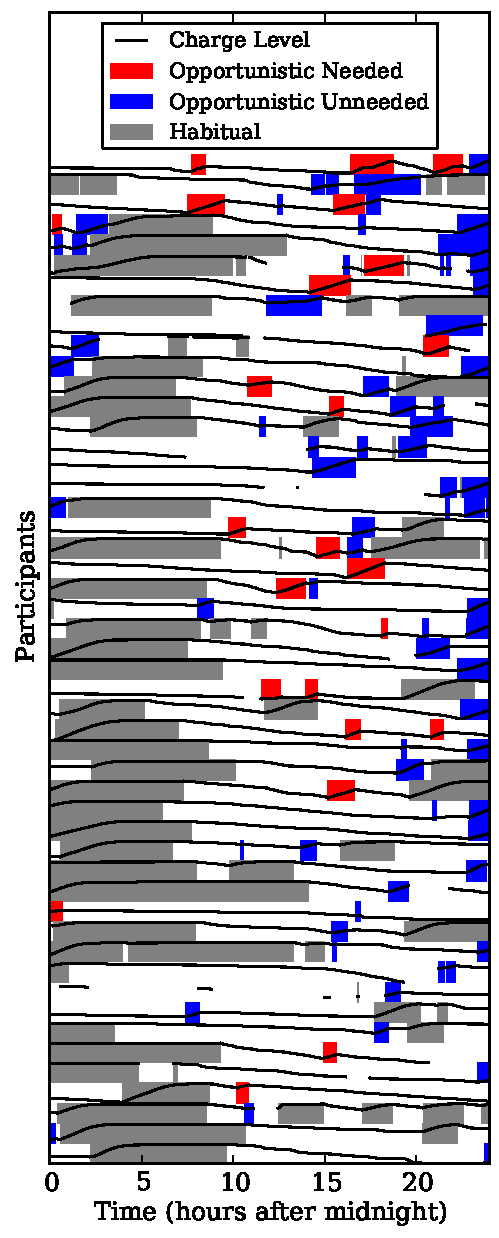
\includegraphics[width=0.7\columnwidth]{./figs/opportunistic.pdf}
\caption{\textbf{Patterns of opportunistic charging.} Many users perform
opportunistic charging multiple times during the day.}
\label{fig-opportunistic-patterns}
\end{figure}

Opportunistic charging may be a response to an anticipated need for more
smartphone battery power: the student who plugs her smartphone in for a brief
charge before a night out. Our data also allowed us to examine how many of
these opportunistic charging sessions were necessary to bridge the gap to the
next full charge. We found that 24 of the 96 (25\%) of the opportunistic
charges we observed were necessary. We believe that this indicates that
participants have responded to their smartphones' battery limitations by
engaging in conservative charging behavior, grabbing power whenever possible
even if they do not anticipate needing it later.

\section{Conclusions}

This abstract introduced \PhoneLab{}, a new large-scale programmable smartphone
testbed operated by SUNY Buffalo and presented the participant behavior in terms
of network transitions, energy, and charging.


{\footnotesize \bibliographystyle{abbrv}
\bibliography{paper}}

\end{document}
